\chapter{Estado da Arte}

\todo{rever}
%A presente seção se encontra divida em uma introdução a programação de
%agentes na seção~\ref{AOP}, onde é discutido o paradigma e os termos agentes
%e personagens. Na seção~\ref{CA:1} a área de computação afetiva é
%apresentada.  O conceito de ontologia é debatido na seção~\ref{onto} e os
%trabalhos relacionados são apresentados na seção~\ref{TR}.

\section{Conceitos de Agente}

\citet{laird2001human} afirmam que a pesquisa em Inteligência Artificial tem
sido fragmentada em muitas áreas especializadas e, assim, algoritmos
específicos e mais eficientes podem ser criados.
%
Há várias definições do conceito de Agente, por exemplo
\cite{shoham1993agent,roadmap,fatemeh2009multi}. \citet{shoham1993agent}
propõe que Agente é uma entidade definida por componentes mentais como
crenças, habilidades, escolhas e comprometimentos.

\citet{franklin1997agent} define um agente através das características que a
entidade deve apresentar.  Atualmente, o menor conjunto comumente aceito
dessas características é composto por três conceitos principais: (i)
Autonomia; (ii) Sociabilidade; (iii) Situacionalidade.
\citet{roadmap,fatemeh2009multi} concordam que autonomia é quando um Agente
toma suas próprias decisões independente de qualquer outra entidade do sistema
ou, ainda, da intervenção diretas de seres humanos. A característica de
sociabilidade permite flexibilidade na execução das tarefas, através da
interação com outros agentes que estejam presentes no sistema. A última,
permite que o agente situe-se em um ambiente dinâmico interagindo com o mesmo
através de algum tipo de sensor ou atuador.

\citet{ingrand1992architecture} indicam que entidades autônomas podem ter a
capacidade de expor seus dados internos para que seja possível um usuário,
possivelmente humano, dar dicas sobre a forma de resolução dos problemas sendo
enfrentados. Esta visão não conflita com a noção de autonomia exposta acima,
pois o agente permanece independente para tomar suas decisões podendo rejeitar
as dicas ou sugestões enviadas pelo usuário.

\citeauthor{ingrand1992architecture} também define Agente em um ambiente com
componentes heterogêneos e com diferentes tempos de resposta para a execução
de suas tarefas. \citet{doyle1998annotated} estendem o conceito dizendo que os
objetos pertencentes ao ambiente devem conter anotações que determinam a forma
de uso dos objetos disponibilizados neles. Assim, não se sabe como todos os
objetos funcionam e, sim, uma forma de aprender com o próprio objeto a sua
forma de utilização. \citet{shoham1993agent} define sociabilidade como uma
habilidade cognitiva necessária para o desempenho das suas tarefas.

Essas inúmeras definições do termo Agente não permite saber se ele é um ser
físico ou abstrato. Dessa forma, \citet{nareyek2001review,damiano2008emotions}
defendem que o agente é o ser abstrato de um ator físico. Em outras palavras,
o ser que age ou atua no meio é chamado de personagem ou ator. Enquanto a
mente desse ser é chamada de agente.

\section{Paradigma de Programação Orientada a Agentes}

\citet{shoham1993agent} propôs em seu trabalho a linguagem \emph{Agent-0} uma
das primeiras a serem baseadas em atos de fala e uma nova visão para se
programar.  Esses atos de fala podem ser vistos como comandos falados entre
atores com as mais diversas finalidades (informar, perguntar, requerer,
aceitar, etc).  Dessa forma, \citeauthor{shoham1993agent} tentou promover a
idéia de computação com uma interação mais social entre membros de um sistema.
Em outras palavras, esse novo paradigma de programação precisa que exista
cooperação e competição entre os agentes para a realização das tarefas
desejadas.

Assim, o agente encontra-se situado em um ambiente no qual pode receber
informações de outros agentes, assim como enviar para outros.  As ações são
estabelecidas utilizando regras que descrevem comportamentos. Assim, é
possível, a própria entidade decidir qual ação deve ser tomada. Essas regras
são construídas em fórmulas lógicas descrevendo-se o contexto que torna um
curso de ação válida e sua consequência que é o conjunto de ações a serem
desempenhadas.

Atualmente, há diversas linguagens para a programação de agentes, por exemplo:
\emph{2APL}, \emph{Agent-0}, \emph{AgentSpeak(L)}, \emph{GOAL} e
\emph{MetateM}~\cite{bordini2009multi}. Elas são baseadas em diversos
formalismos diferentes. MetateM por exemplo é baseada em lógica temporal,
permitindo que formulas temporais definindo o comportamento do agente sejam
diretamente executadas.

A plataforma \jason \cite{bordini-jason} utilizada no trabalho pode ser
pensada como um sistema de planejamento reativo, em que planos são executados
a partir de alterações nas crenças e objetivos do agente. A plataforma
baseia-se na arquitetura BDI e utiliza uma extensão da linguagem de
programação abstrata, definida por \citet{rao1996agentspeak}, chamada
AgentSpeak(L), para especificar o reciocínio sobre ações dos agentes. A grande
vantagem dessa plataforma é a rapidez com que melhorias têm sido feitas e a
facilidade de customização de diversos componentes da plataforma.

\section{Computação Afetiva}

\citet{Pic98} definiu Computação Afetiva como uma ``computação relacionada,
surgida ou que influência as emoções''. Além disso, computadores com emoções
permitem aos mesmos um determinado nível de comportamento inteligente e
criatividade que seria impossível sem as emoções e esse é o principal desafio
dessa área. Logo, o seu entendimento pode explicar fenômenos como, por
exemplo, atenção, memória e outros.


Essa área é normalmente dividida em duas sub-áreas. A primeira estuda o
reconhecimento e a expressão de emoções dentro da Interação Homem-Computador;
a segunda, foca na síntese de emoções para aprimorar os seres robóticos e/ou
para estudar o comportamento humano por meio de simulações. Há muita
aplicabilidade dessas técnicas, por exemplo: a área que reconhece as emoções
pode ser utilizada para adaptar o sistema ao estado da pessoa permitindo ao
mesmo instruí-la, questioná-la, encorajá-la ou ocultar determinadas
informações consideradas irrelevantes.

O objetivo de \citet{bick2003relational} com o projeto \emph{Relational
Agents} é possibilitar aos usuários a criação de um relacionamento social e
emocional com longa duração.  Em \citet{bickmore2009virtual}, a confiança no
agente torna possível discutir tarefas mais importantes como melhoria da saúde
ou até a compra de uma casa. Outro trabalho na área de IHC é o reconhecimento
de emoções para aumentar a imersão em jogos, por exemplo permitindo ao próprio
jogo adaptar eventos ou trechos tornando-o mais divertido e realista.

\begin{figure}
  \begin{center}
    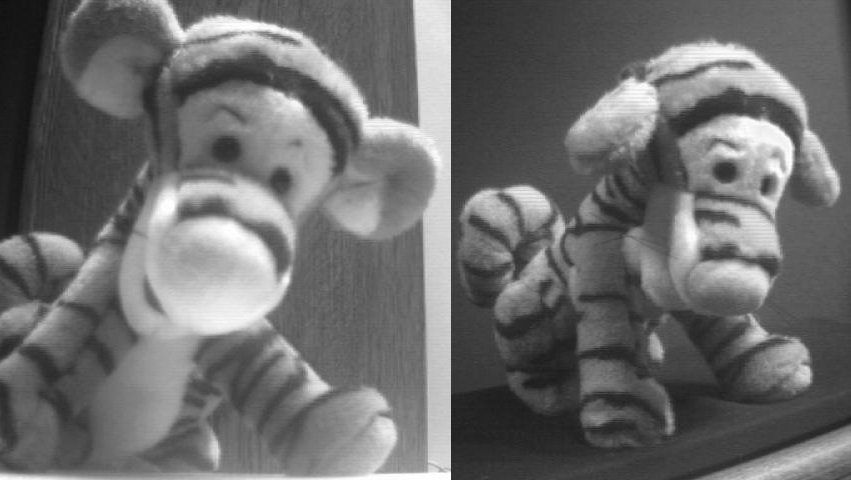
\includegraphics[width=75mm]{figuras/tigger-mit.png}
  \end{center}
  \caption{Brinquedo que responde as emoções das crianças \cite{kirsch1999affective}.}
  \label{fig:tigger-mit}
\end{figure}

O projeto \emph{The Affective Tigger: a reactive expressive toy} de
\citet{kirsch1999affective} é um brinquedo capaz de reconhecer e reagir às
emoções exibidas pelas crianças. Por exemplo, quando a criança encontra-se
feliz, o boneco expressa felicidade (ver Figura~\ref{fig:tigger-mit}). Ao todo
existem 5 estados emocionais: muito feliz, feliz, neutro, triste e muito
triste. Todos, com exceção do neutro, possuem alguma síntese vocal como um
rosnado (tristeza) ou uma risada (muito feliz). Assim, esse brinquedo, por ser
considerado um ser robótico que reage à criança com seus próprios estados
emocionais, fica enquadrado na segunda área.  Portanto, o desenvolvimento
desse brinquedo serviu para aprimorar os seres robóticos.

O projeto AIDA\footnote{Mais detalhes, ver http://senseable.mit.edu/aida} (do
inglês \emph{Affective Intelligent Driving Agent}) pode ser entendido como
enquadrado na área de IHC, pois o interesse é entender o estado afetivo da
pessoa dirigindo. Além disso, interessa-se em ter um relacionamento com o
usuário sugerindo alterações nas rotas baseado na rotina aprendida depois de
um mês de aprendizado.  A pesquisa relatada em \citet{dias-agents} visou
melhorar a simulação de agentes através do uso da emoção guiando o processo
deliberativo e melhorar o entendimento e gerência das emoções.  O presente
trabalho se enquadra na área de síntese de emoção, pois o interesse é em
entender o estado emocional e como ele pode afetar o comportamento de um
personagem.

\section{Modelo Psicológico de Emoção}

Segundo \citet{scherer2000tnoe}, na psicologia há diferentes modelos para
tentar mapear a afetividade: dimensionais, discretos, baseados em significados
e componentes. Os modelos dimensionais procuram estabelecer eixos de classes
de emoções e formas de se mover por esses.  Enquanto os modelos discretos
visam descrever um conjunto básico de emoções ou, ainda, um sistema adaptativo
que evolua a partir de um determinado ponto.  Os modelos baseados em
significados constroem estruturas semânticas e descrevem verbalmente o que
ocorre em determinado sentimento; em outras palavras, preocupa-se com as
situações em que ocasionaram o mesmo. Já os modelos baseados em componentes
entendem que emoções são aprendidas e, sendo assim, estudam o elo entre os
sentimentos e os eventos ou situações que as mesmas acontecem. Esse elo é
montado pela pessoa de diferentes formas.

\citet{Pic98} chama atenção que as emoções sempre foram consideradas um
estigma pela ciência que é fundamentalmente racional com hipóteses testáveis,
argumentos lógicos e experimentos repetitivos.  Entretanto, estudos
neurológicos recentes \cite{ledoux1998emotional,damasio2004erro} mostram a
importância das emoções na tomada de decisão.  \citet{damasio2004erro}
diferencia emoção de sentimento; para ele emoção é um estado físico do corpo e
sentimento é a percepção da mudança desse estado corporal.

\begin{figure*}
  \centering
    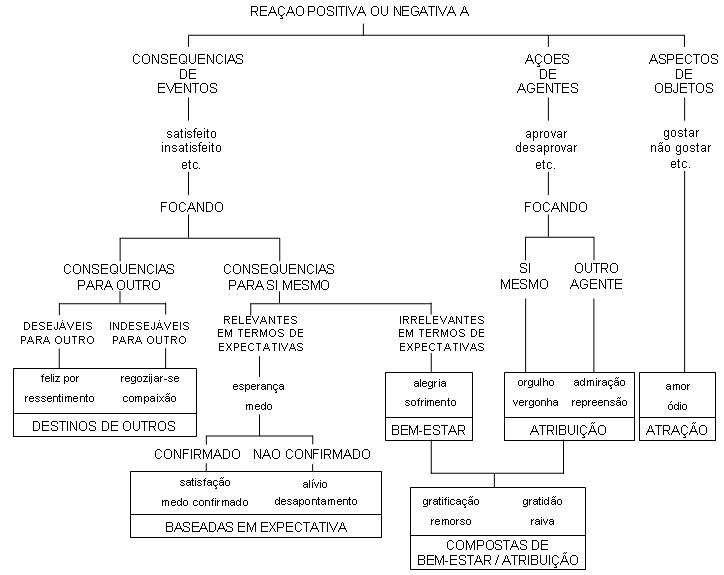
\includegraphics[width=150mm]{figuras/pontarolo_occ.png}
  \caption{Modelo OCC adaptado de \cite{pontarolo2008modelagem}.}
  \label{fig:occ_model_original}
\end{figure*}

O modelo proposto por \citeauthor*{ortony1988cse} \cite{ortony1988cse},
conhecidos na comunidade de Inteligência Artificial, é chamado de OCC por
causa de seus autores.  Esse modelo é classificado como baseado em
significados por descrever as situações de ocorrências de cada uma de suas 22
emoções.  Essas emoções são divididas em formas de se perceber o mundo a sua
volta: Eventos (importantes para alguma meta), Agentes (incluindo a si mesmo)
e Objetos (atração ou repulsa). Assim sendo, essas maneiras de se perceber o
mundo refletem diferentes jeitos de se analisar as situações que podem ser
relativas aos objetivos, valores morais ou gostos da pessoa.

A Figura~\ref{fig:occ_model_original} resume o modelo OCC e mostra as
percepções possíveis de um indivíduo.  Partindo da direita para esquerda, o
ramo mais básico, Aspectos de Objetos, é ativado quando se avalia o gosto de
alguém para algum objeto (inanimado ou não), por exemplo, alguém gostar de
rosas vermelhas.  No seguinte, Ações de agentes, o julgamento das ações
exercidas por outro indivíduo é realizado baseado nos valores morais da pessoa
que está julgando.  Sendo assim, por exemplo, reprovar a atitude de um colega
que ``colou'' na prova. O último da árvore, mais a esquerda, é o de evento que
representa as coisas que aconteceram (e foram consideradas importantes),
acontecem e acontecerão (objetivos almejados). Esses são avaliados segundo as
suas consequências para o alcance ou impedimento dos objetivos de uma pessoa.
Por exemplo, preciso ir bem no concurso para ficar satisfeito porque esse
evento me permitirá alcançar minha meta de ser contratado.

Ainda segundo o modelo OCC, as emoções possuem intensidades. Entretanto, há
distinção entre a valência da emoção e a valência do sentimento. No modelo, um
indivíduo só possui o sentimento quando a intensidade da emoção ultrapassar um
determinado limite.  Essa intensidade é obtida por uma função matemática que
utiliza variáveis de dois tipos: local, que influencia as emoções em um ramo
específico; e global, que influencia todas as emoções do indivíduo.  Um
exemplo de variável local é o desejo, enquanto que um exemplo de variável
global é o senso de realidade.

\section{Ontologias}

\todo{reescrita} Desde Aristóteles, de acordo com \citet{wks2008towards},
começa o estudo das coisas existentes no mundo e a natureza desse existência,
um ramo da filosofia conhecido com ontologia.  Atualmente, na ciência da
computação, ontologias são vistas como um vocabulário de entendimento comum e
compartilhado de um domínio que pode ser utilizada para comunicação entre
pessoas e aplicações distribuídas e heterogêneas.  \citet{ontoly2004Approach}
definem ontologia como uma representação de conhecimento utilizada para
capturar conhecimento e informação sobre determinado assunto, geralmente
estruturado de forma similar a uma rede semântica. Sendo assim, uma ontologia
consiste de um diagrama composto de nodos e arcos que estabelecem uma
fundamentação semântica que permite melhorar a descoberta, interoperabilidade
e reuso do conhecimento.

Logo, o conhecimento pode ser usado de maneiras diferentes e não serve somente
para conter informações em categorias, mas também serve como um tipo de
``banco de dados'' onde instâncias são armazenadas e recuperadas.  O tipo ou
classe da informação possui propriedades que diferem da sua instância. Essa
diferença fica clara quando é feita a comparação da ontologia com uma base de
dados, onde as classes de informações definidas criam as tabelas e as
instâncias povoam os dados nas tabelas.

Na área da computação, ontologias ganharam maior importância com a Web
Semântica permitindo que o conhecimento da página seja facilmente obtido sem
um processamento pesado.  A W3C, orgão internacional que regulamenta padrões
utilizados na Web, regulamentou diversos padrões baseados em \emph{XML} para
ontologias.  A linguagem que será utilizada no presente trabalho será a
OWL\footnote{A sigla vem de ``\emph{Ontology Web Language}''.} e esta fora do
escopo desse artigo aborda-lá em detalhes \footnote{Para mais detalhes, veja
\url{http://www.w3.org/standards/semanticweb/ontology}.}.

\section{Ontologias afetivas}
...

\section{Ontologias de Humanos Virtuais}
...

\section{Trabalhos Relacionados}

O comportamento emotivo do personagem tem um papel importante para se ter a
ilusão de vida conforme afirmou \citet{bates1994role}. Esse trabalho utiliza o
modelo OCC para melhorar a credibilidade dos agentes e cada uma das emoções
pode ser ligada a um comportamento. No exemplo dado anteriormente, um agente
pode ligar o medo a um comportamento agressivo enquanto outro liga essa mesma
emoção de medo a um comportamento de estado alarmado.

\citet{GraCli98} criaram um mecanismo evolucionário utilizando redes neurais
com uma base química para guiar o comportamento do ator. Os atores simulados
podem envelhecer, aprender e, inclusive, se reproduzir (aqui são utilizados
algoritmos genéticos).  Por exemplo, o personagem pode aprender algumas
palavras básicas e demostrar que esta envelhecendo por meio da mudança da cor
de seus cabelos dando uma certa ilusão de vida.

Conforme já dito, as emoções podem melhorar a credibilidade dos seres
virtuais.  \citet{zhang2009emotional} desenvolveram uma aplicação com a
finalidade de demostrar esse conceito. O planejamento das ações a serem
executadas pelo personagem é afetado pelos valores das emoções sendo
experimentadas.

Todos os trabalhos apresentados até aqui, utilizaram as emoções para aumentar
a representação ou expressividade de um ator. Entretanto,
\citet{neto2010construction} tentam estudar o impacto da emoção na decisão dos
agentes.  Assim, para isso ser possível, foi necessário alterar a forma de
planejamento das decisões, além de como recuperar os dados da sua memória.  A
modificação no acesso a memória permite o ``esquecimento'' de determinadas
crenças quando o estado emocional for diferente daquele guardado junto da
memória a ser recuperada. Essa característica torna o planejamento do agente e
as atitudes dos personagens mais realísticas.

\citet{benta2007ontology} e \citet{wks2008towards} descrevem modelos afetivos
através de ontologias. No primeiro trabalho, uma ontologia foi criada
descrevendo emoções primárias e secundárias. O primeiro tipo de emoção exige
menos processamento cognitivo que o segundo. Além disso, o modelo descreve ao
todo 11 emoções sendo 7 dessas consideradas primárias.

